\chapter{IPv6}
Eine IPv6-Adresse ist eine 128 Bit Zahl. Es gibt $2^{128}$ IPv6-Adressen ($340\cdot10^{36}$).

\textbf{Schreibweise einer IPv6-Adresse} \\
\begin{itemize}
	\item Hexadezimale Schreibweise (32 Zeichen)
	\item Gruppen von 16 Bit mit : getrennt
	\item Führende Nullen werden in jeder Gruppe weggelassen
	\item Einmalig kann der längste Block an Nullen mit :: ersetzt werden
\end{itemize}

Bsp: \\
2001:ABAD:0000:0430:0000:0000:00C9:0001 \\
2001:ABAD:0:430:0:0:C9:1 \\
2001:ABAD:0:430::C9:1

\textbf{Subnetzmaske}
\begin{itemize}
	\item trennt in Netz- und Hostteil 
	\item nur noch Präfix-Notation
	\item Es wird fast nur /64 verwendet
\end{itemize}

\textbf{Idee von IPv6}
\begin{itemize}
	\item mehr IP-Adressen
	\item Problem: alle Protokolle die IPv4 verwenden müssen erneuert werden
	\item Alte Fehler/Security-Probleme beheben
	\item leichterer Header
\end{itemize}

\textbf{Übergang von IPv4 zu IPv6}
\begin{itemize}
	\item Dualer Stack
	\item Translation
	\begin{figure}[H]
		\centering
		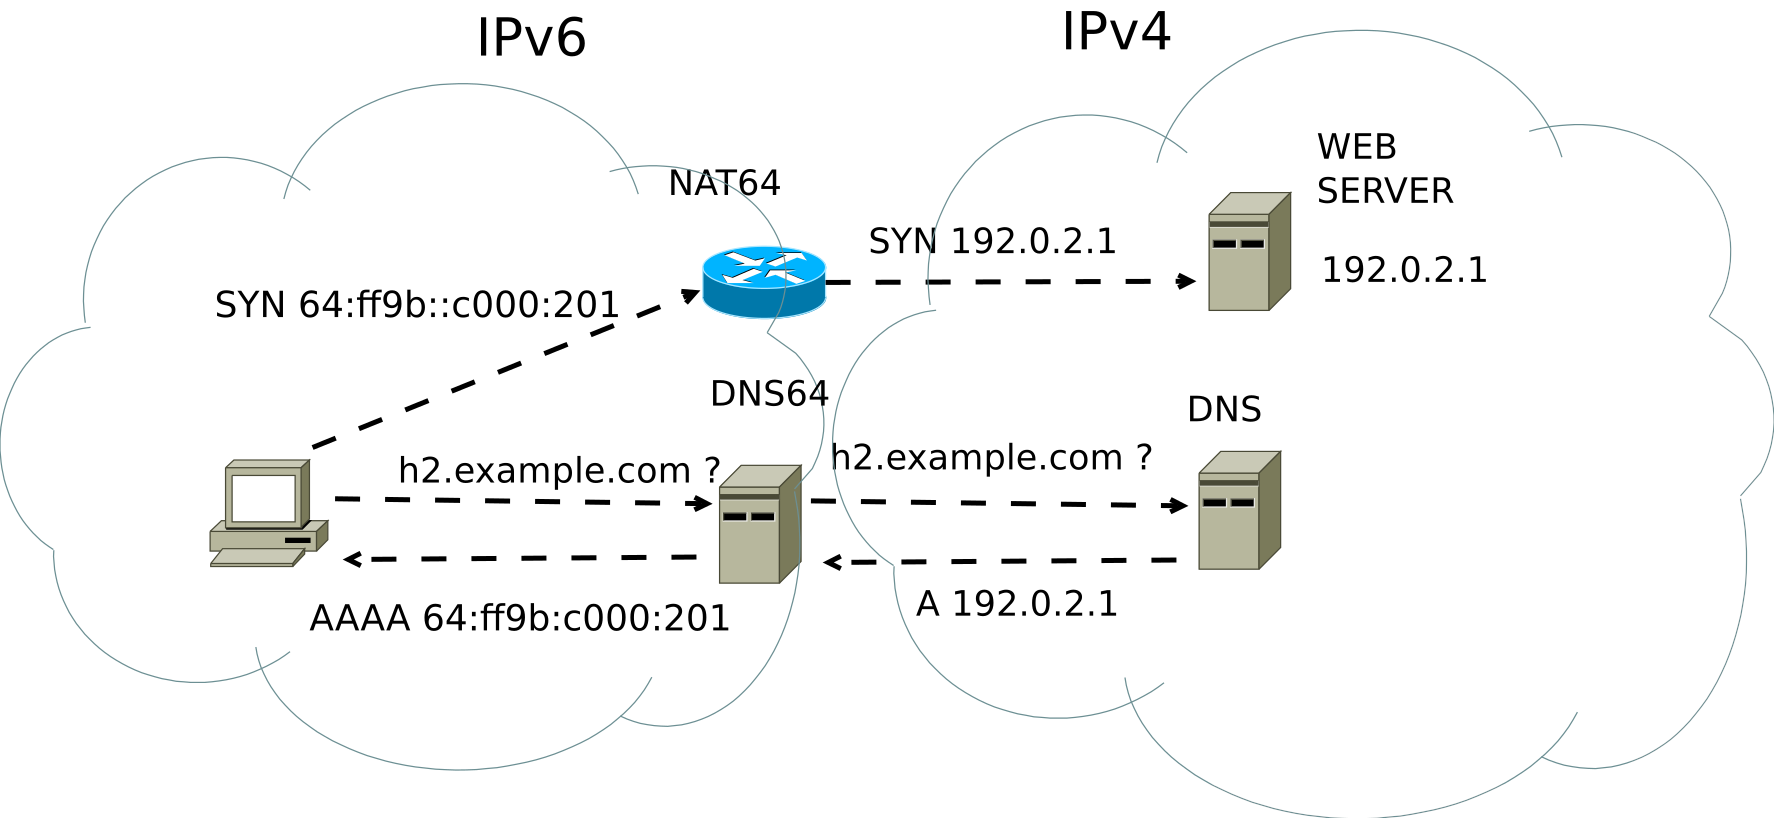
\includegraphics[width=0.7\linewidth]{figures/nat64.png}
		\caption{IPv4-IPv6 Translation mit NAT64}
	\end{figure}
	\item Tunneling
		\begin{figure}[H]
		\centering
		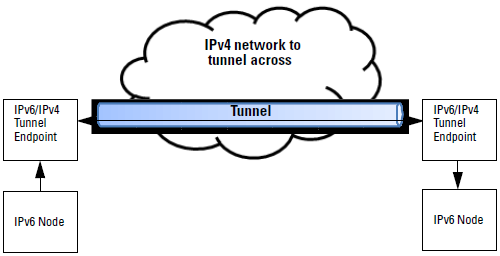
\includegraphics[width=0.7\linewidth]{figures/ipv6_tunneling.png}
		\caption{IPv4-IPv6 Tunneling}
	\end{figure}
\end{itemize}

\textbf{Kommunikationsarten}
\begin{itemize}
	\item Unicast
	\item Multicast \\
	ff02::1 ... all-nodes-multicast (Broadcast) \\
	ff02::2 ... all-router-multicast
	\item Anycast (der 'nägeste' einer Gruppe bekommt den Anycast)
\end{itemize}

\textbf{IPv6-Unicast Adressen} \\
\begin{itemize}
	\item Global Unicast Adressen 2000-3fff (vgl. öffentliche IP)
	\item Link Local Adressen fe80-febf (für das lokale Netz, nicht routbar)
	\item loopback ::1 (vgl. IPv4 127.0.0.1)
	\item Unspecified Adress :: (vgl. IPv4 0.0.0.0)
	\item Unique Local fc00-fdff (vgl. IPv4 NAT)
	\item Embedded IPv4
\end{itemize}

\textbf{IP-Konfiguration}
\begin{itemize}
	\item statisch (GUA, LLA)
	\item dynamisch
	\begin{itemize}
		\item SLAAC
		\item SLAAC mit stateless DHCPv6 Server
		\item DHCPv6
	\end{itemize}
\end{itemize}

\textbf{SLAAC} \\
\begin{figure}[H]
	\centering
	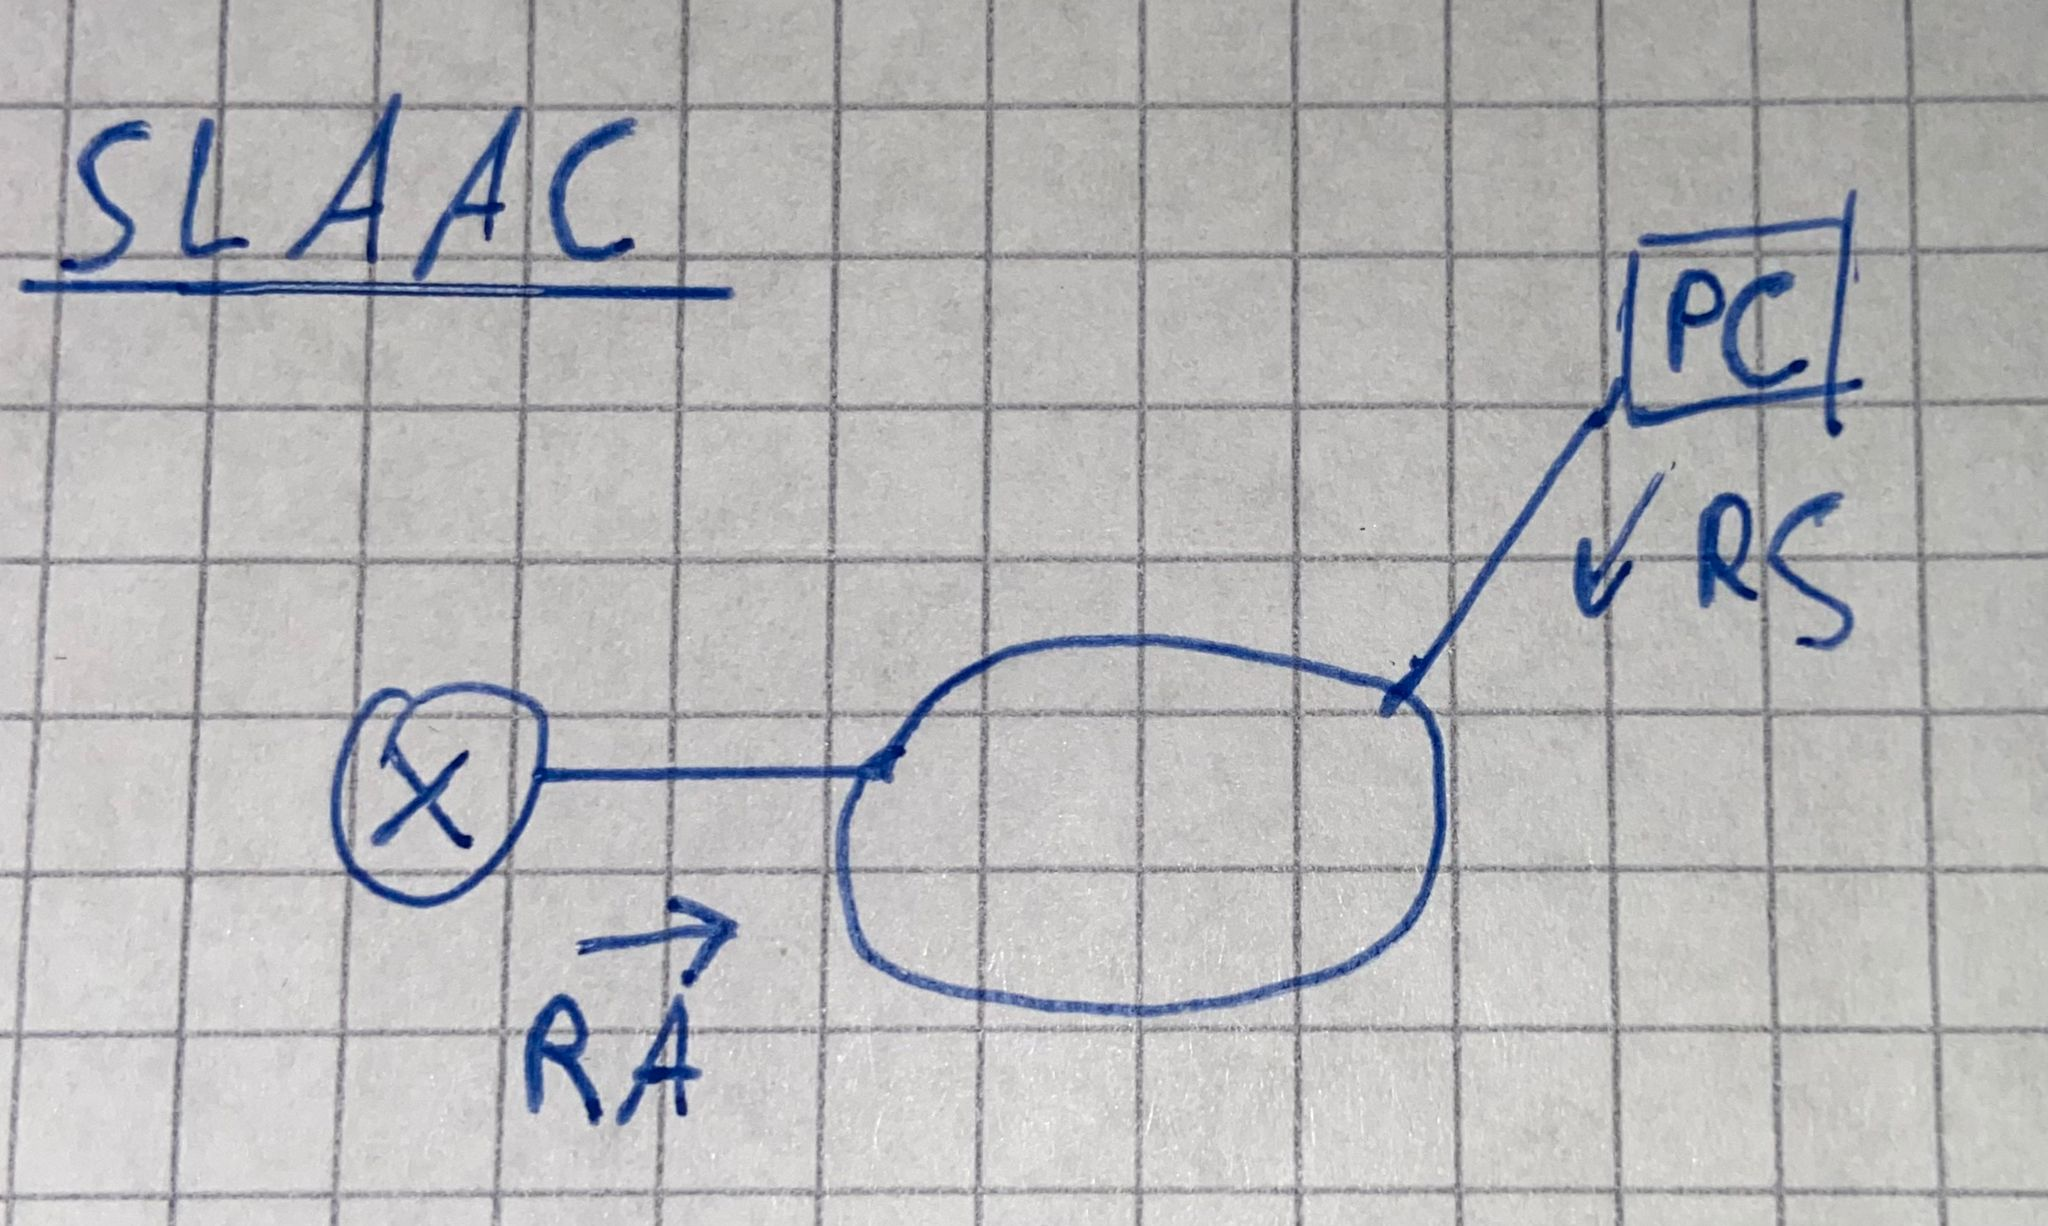
\includegraphics[width=0.8\linewidth]{figures/slaac.jpeg}
	\caption{SLAAC}
\end{figure}
Router senden (ca. alle 200s) ein RA-Paket (Router Advertisement) aus. Dies enthält die wichtigsten Informationen für die Hosts (Präfix, Präfix-Länge, Default-Gateway). Die Hosts geben sich dann selbst die IPv6-Adresse. \\
Hostteil
\begin{itemize}
	\item Zufallszahl (ND-Protokoll)
	\item EUI-64 (MAC-Adresse)
\end{itemize}
Die Hosts können RS (Router Solicitation) Pakete aussenden um das RA-Paket anzufordern.



